\documentclass[12pt,a4paper]{article}
\usepackage{geometry}
\usepackage{graphicx}
\usepackage{listings}
\usepackage{xcolor}
\usepackage{hyperref}
\usepackage{fancyhdr}
\usepackage{float}
\usepackage{longtable}
\usepackage{url}

\geometry{a4paper, margin=1in}

\graphicspath{{./Screenshots/}}

\definecolor{codebg}{rgb}{0.95,0.95,0.95}
\lstset{
    backgroundcolor=\color{codebg},
    basicstyle=\ttfamily\small,
    breaklines=true,
    numbers=left,
    tabsize=4,
    language=Python
}

\pagestyle{fancy}
\fancyhf{}
\fancyhead[L]{Comp 2322 Computer Networking}
\fancyhead[R]{Project Report}
\fancyfoot[C]{\thepage}

\begin{document}

\begin{titlepage}
    \centering
    \vspace*{3cm}
    {\Large \textbf{COMP 2322 Computer Networking}}\\[0.5cm]
    {\LARGE \textbf{Multi-thread Web Server}}\\[0.5cm]
    {\large Project Report}\\[2cm]
    
    \begin{tabular}{ll}
        \textbf{Name:} & Meng Zihan \\
        \textbf{Student ID:} & 24110285D \\
        \textbf{Email:} & 24110285d@connect.polyu.hk \\
        \textbf{Date:} & April 20, 2026 \\
    \end{tabular}
    
    \vfill
    {\small The Hong Kong Polytechnic University}
\end{titlepage}

\tableofcontents
\newpage

\section{Overview}
This project implements a multi-threaded web server from scratch using Python socket programming. Server runs on port \textbf{8848}.

\subsection{Project Structure}
\begin{verbatim}
project/
├── report/
│   ├── report.tex
│   └── Screenshots/
│       ├── 01_server_startup.png
│       ├── 02_stage1_request.png
│       ├── 03_get_text.png
│       ├── 04a_get_image_browser.png
│       ├── 04b_get_image_curl.png
│       ├── 05_head_method.png
│       ├── 06_404_not_found.png
│       ├── 07_403_forbidden.png
│       ├── 08_400_bad_request.png
│       ├── 09_10_lastmod_304.png
│       ├── 11_12_keepalive_close.png
│       ├── 13_concurrent_load.png
│       ├── 14_access_log.png
│       └── 15_status_dashboard.png
├── server.py
├── webs/
│   ├── index.html
│   └── test.jpg
├── logs/
│   └── server.log
└── test.ipynb
\end{verbatim}

\section{Design Highlights}

\subsection{Producer-Consumer Thread Model}
Main thread acts as dispatcher, only accepting connections. Worker threads handle requests independently. This prevents slow requests from blocking new connections.

\subsection{Short-Circuit Cache Validation}
Server checks If-Modified-Since before reading files. If unchanged, returns 304 immediately, skipping disk I/O and network transmission.

\subsection{Two-Layer Path Traversal Protection}
\begin{enumerate}
    \item \texttt{os.path.normpath()} normalizes malicious paths
    \item \texttt{os.path.realpath()} prefix verification ensures file stays within web root
\end{enumerate}

\subsection{Structured Logging}
Pipe-separated format enables easy parsing: \texttt{ip | timestamp | request | status}

\subsection{Zero-Config Startup}
Server auto-creates webs/, logs/, and default index.html on first run.

\section{Implementation - Three Stages}

\subsection{Stage 1: Basic Socket Server}
Simple TCP server that accepts connections and returns a fixed response.

\begin{lstlisting}[caption=Basic Server Loop]
def main():
    server_socket = socket.socket(socket.AF_INET, socket.SOCK_STREAM)
    server_socket.bind(('127.0.0.1', 8848))
    server_socket.listen(5)
    while True:
        client_socket, addr = server_socket.accept()
        data = client_socket.recv(4096)
        client_socket.send(b"HTTP/1.1 200 OK\r\n\r\nHello")
        client_socket.close()
\end{lstlisting}

\subsection{Stage 2: File Serving}
Added file reading, MIME types, and status codes (200, 404, 403).

\begin{lstlisting}[caption=File Serving]
file_path = os.path.join('webs', path.lstrip('/'))
if os.path.exists(file_path):
    with open(file_path, 'rb') as f:
        content = f.read()
    send_response(200, content)
else:
    send_response(404, "Not Found")
\end{lstlisting}

\subsection{Stage 3: Multi-threading \& Advanced Features}
\begin{itemize}
    \item Each request handled in separate thread
    \item HEAD method support
    \item Logging to logs/server.log
\end{itemize}

\begin{lstlisting}[caption=Multi-threading]
threading.Thread(target=handle_client, args=(client_socket, addr)).start()
\end{lstlisting}

\section{Additional Features}

\subsection{Cache Validation (304)}
Server returns Last-Modified header. If client sends If-Modified-Since and file unchanged, returns 304.

\subsection{Keep-Alive}
Same TCP connection reused for multiple requests. Loop continues until Connection: close.

\subsection{Status Dashboard}
Visit \texttt{http://127.0.0.1:8848/status} to see:
\begin{itemize}
    \item Server uptime
    \item Active threads
    \item Total requests
    \item Recent logs
\end{itemize}

\section{Test Results}

\subsection{Test 1: Server Startup}
\textbf{Command:} \texttt{python server.py}

\textbf{Expected:} Server starts on port 8848, creates webs/ and logs/ directories.

\begin{figure}[H]
    \centering
    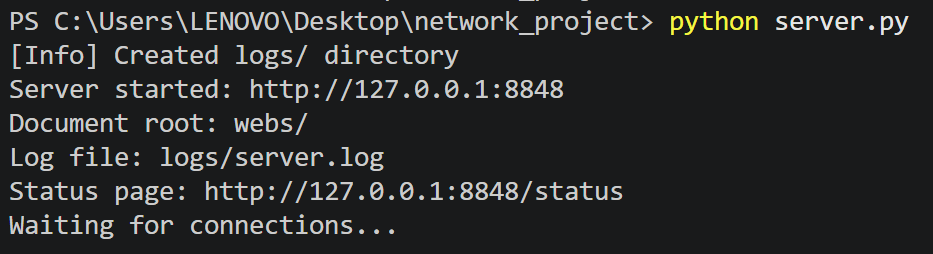
\includegraphics[width=0.8\textwidth]{01_server_startup.png}
    \caption{Server startup}
    \label{fig:startup}
\end{figure}

\subsection{Test 2: Stage 1 Request Display}
\textbf{Command:} Client connects, server displays raw HTTP request.

\textbf{Expected:} Server console shows received HTTP request.

\begin{figure}[H]
    \centering
    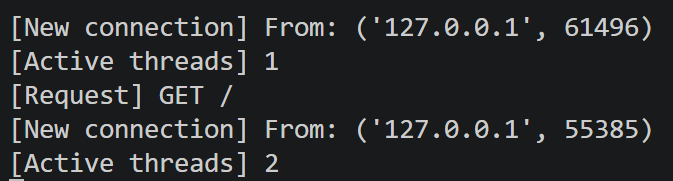
\includegraphics[width=0.8\textwidth]{02_stage1_request.png}
    \caption{Stage 1 - Raw request display}
    \label{fig:stage1}
\end{figure}

\subsection{Test 3: GET Text File}
\textbf{Command:} \texttt{curl http://127.0.0.1:8848/index.html}

\textbf{Expected:} HTTP 200 OK, returns index.html content.

\begin{figure}[H]
    \centering
    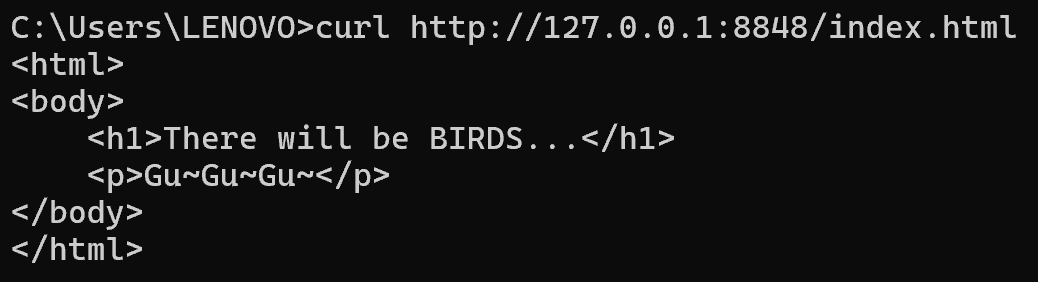
\includegraphics[width=0.8\textwidth]{03_get_text.png}
    \caption{GET text file - 200 OK}
    \label{fig:get_text}
\end{figure}

\subsection{Test 4: GET Image File}
\textbf{Command:} \texttt{curl -I http://127.0.0.1:8848/test.jpg}

\textbf{Expected:} HTTP 200 OK, Content-Type: image/jpeg. Browser displays image.

\begin{figure}[H]
    \centering
    \begin{minipage}{0.48\textwidth}
        \centering
        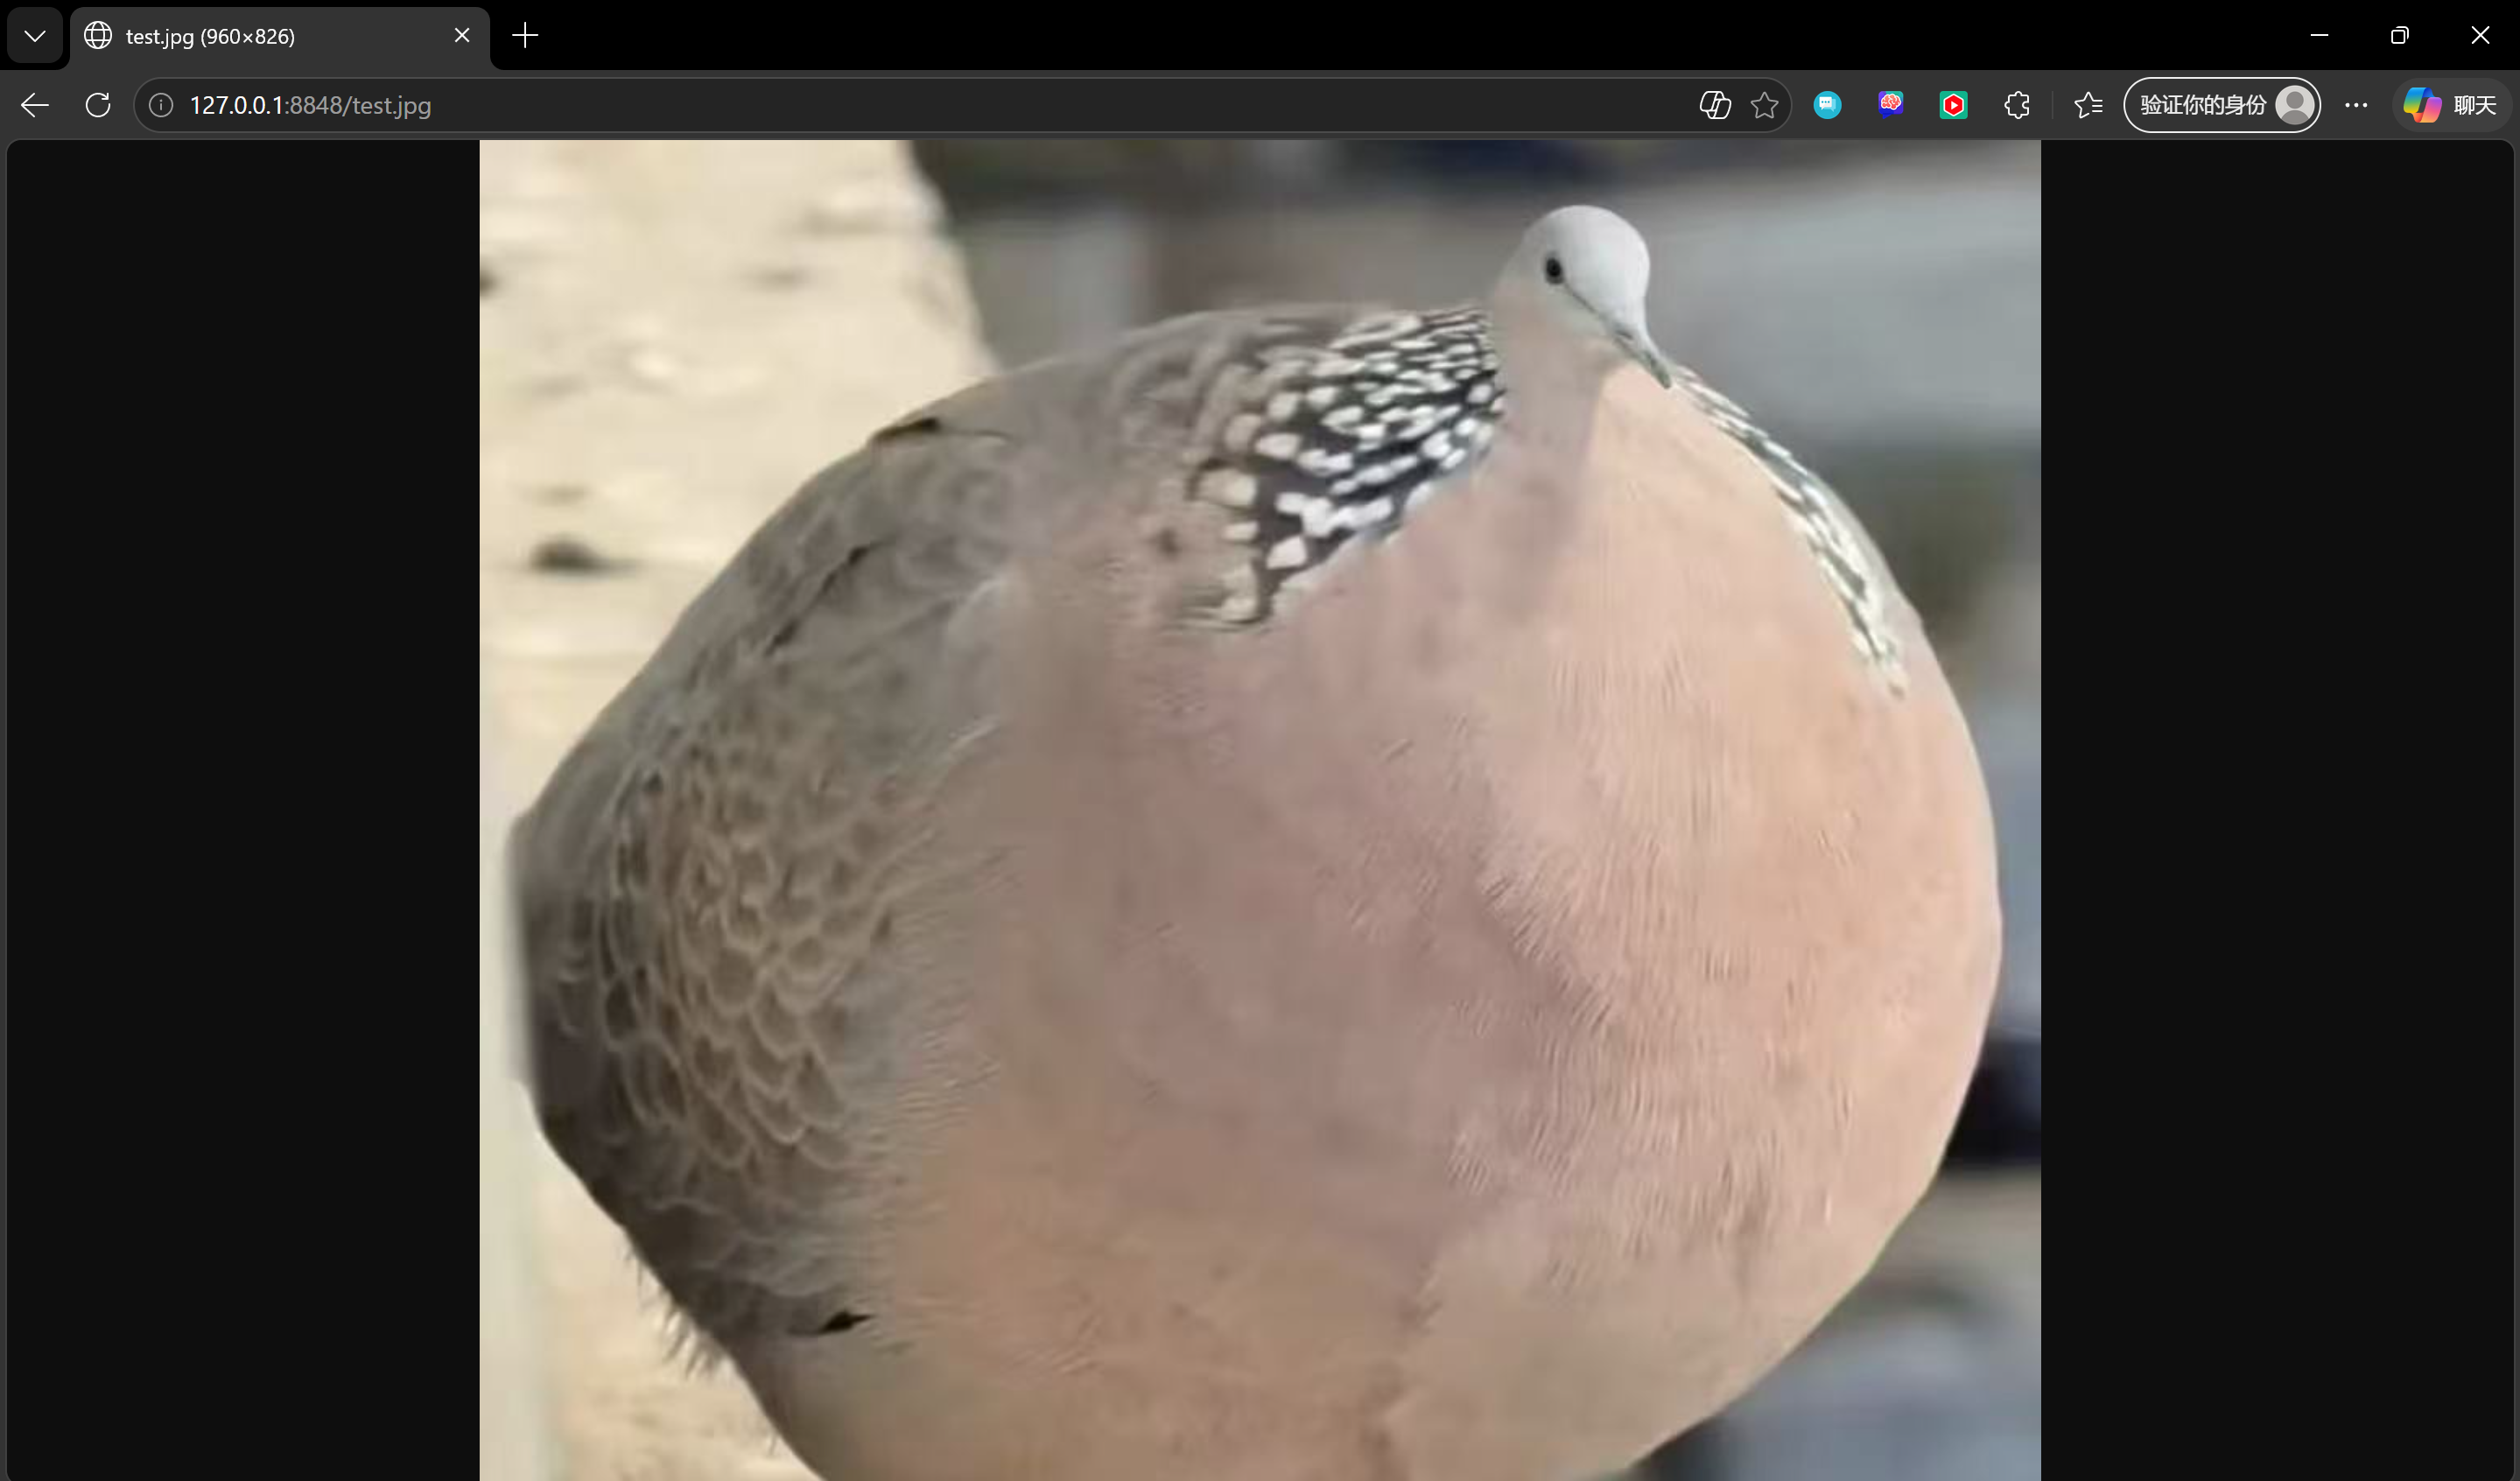
\includegraphics[width=\textwidth]{04a_get_image_browser.png}
        \caption{Browser displaying image (Spotted Dove)}
        \label{fig:dove}
    \end{minipage}
    \hfill
    \begin{minipage}{0.48\textwidth}
        \centering
        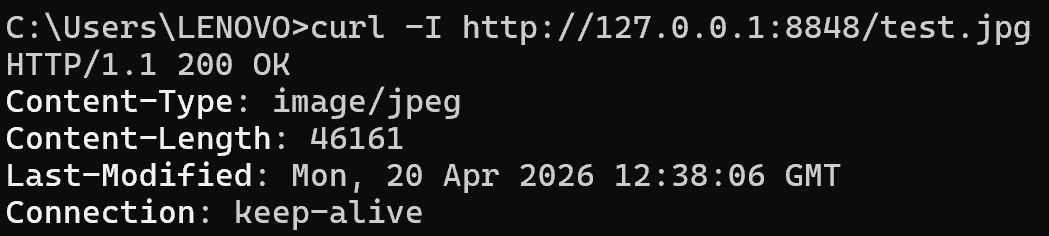
\includegraphics[width=\textwidth]{04b_get_image_curl.png}
        \caption{curl -I: 200 OK, image/jpeg}
        \label{fig:get_image_curl}
    \end{minipage}
\end{figure}

\subsection{Test 5: HEAD Method}
\textbf{Command:} \texttt{curl -I http://127.0.0.1:8848/index.html}

\textbf{Expected:} HTTP 200 OK with headers only, no message body.

\begin{figure}[H]
    \centering
    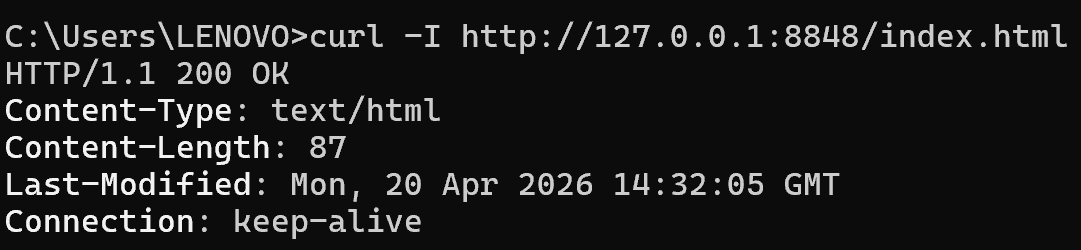
\includegraphics[width=0.8\textwidth]{05_head_method.png}
    \caption{HEAD method - headers only}
    \label{fig:head}
\end{figure}

\subsection{Test 6: 404 Not Found}
\textbf{Command:} \texttt{curl http://127.0.0.1:8848/nonexistent.html}

\textbf{Expected:} HTTP 404 Not Found with error page.

\begin{figure}[H]
    \centering
    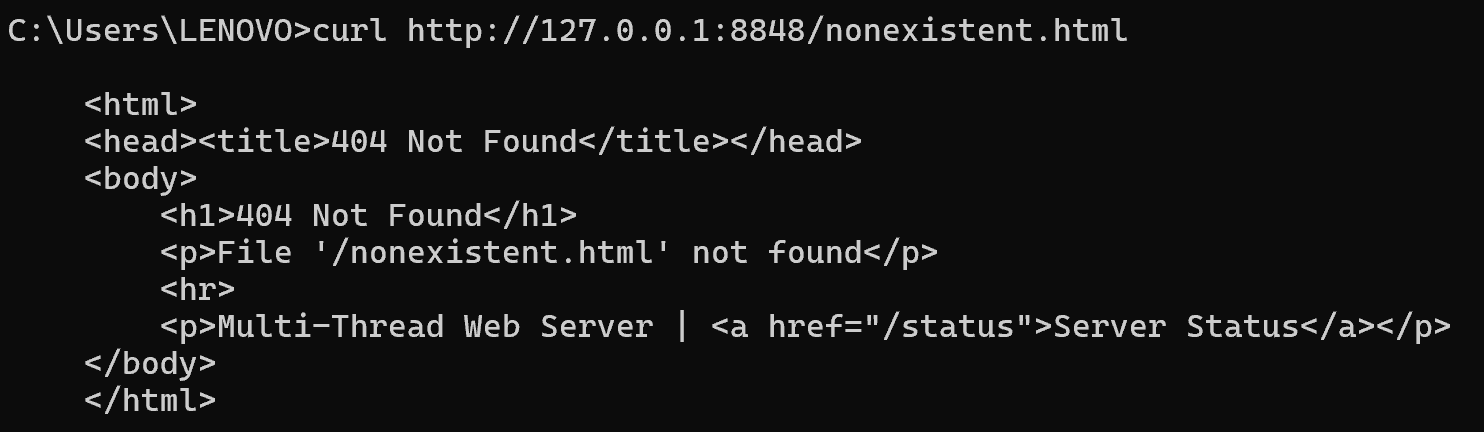
\includegraphics[width=0.8\textwidth]{06_404_not_found.png}
    \caption{404 Not Found}
    \label{fig:404}
\end{figure}

\subsection{Test 7: 403 Forbidden}
\textbf{Command:} \texttt{curl --path-as-is http://127.0.0.1:8848/../server.py}

\textbf{Expected:} HTTP 403 Forbidden (path traversal protection).

\begin{figure}[H]
    \centering
    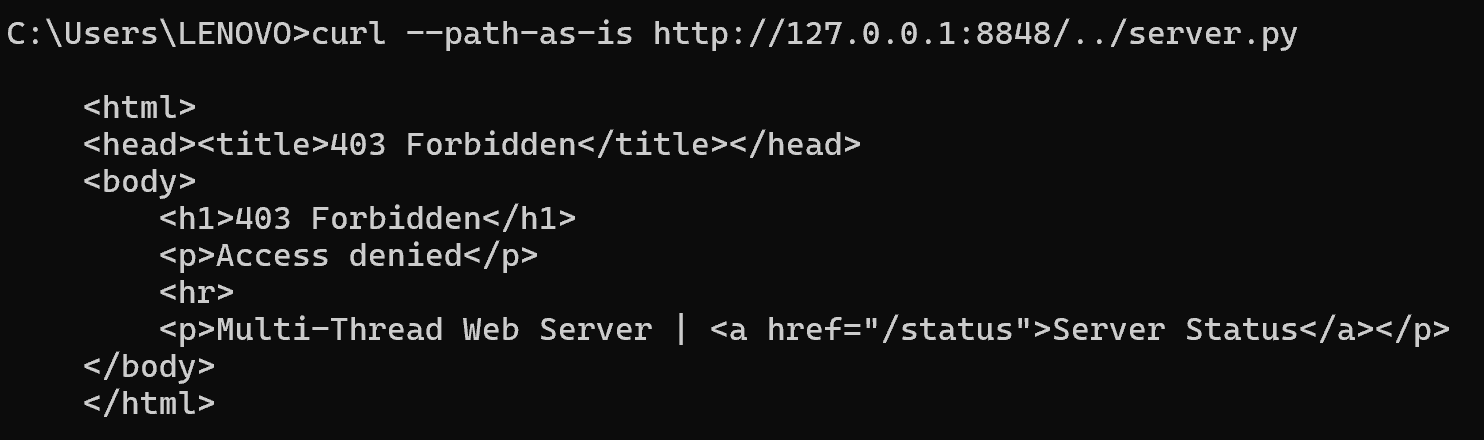
\includegraphics[width=0.8\textwidth]{07_403_forbidden.png}
    \caption{403 Forbidden - path traversal protection}
    \label{fig:403}
\end{figure}

\subsection{Test 8: 400 Bad Request}
\textbf{Command:} Python socket (see Jupyter Notebook Cell 7)

\textbf{Expected:} HTTP 400 Bad Request.

\begin{figure}[H]
    \centering
    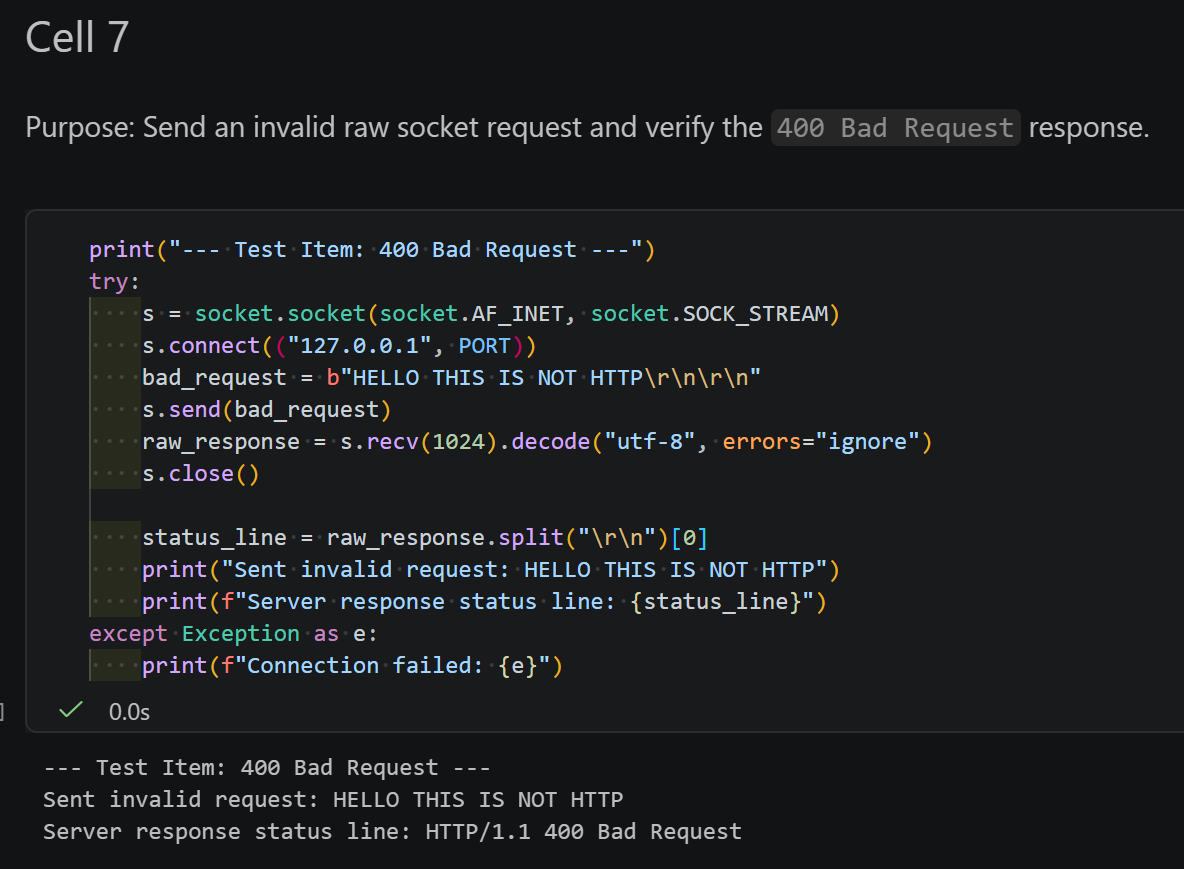
\includegraphics[width=0.8\textwidth]{08_400_bad_request.png}
    \caption{400 Bad Request (Cell 7 output)}
    \label{fig:400}
\end{figure}

\subsection{Test 9-10: Last-Modified and 304 Not Modified}

\textbf{Step 1:} Get Last-Modified header
\begin{verbatim}
curl -v http://127.0.0.1:8848/index.html 2>&1 | findstr "Last-Modified"
< Last-Modified: Mon, 20 Apr 2026 14:50:23 GMT
\end{verbatim}

\textbf{Step 2:} Conditional request with If-Modified-Since
\begin{verbatim}
curl -v --header "If-Modified-Since: Mon, 20 Apr 2026 14:50:23 GMT" http://127.0.0.1:8848/index.html
< HTTP/1.1 304 Not Modified
< Connection: close
\end{verbatim}

\begin{figure}[H]
    \centering
    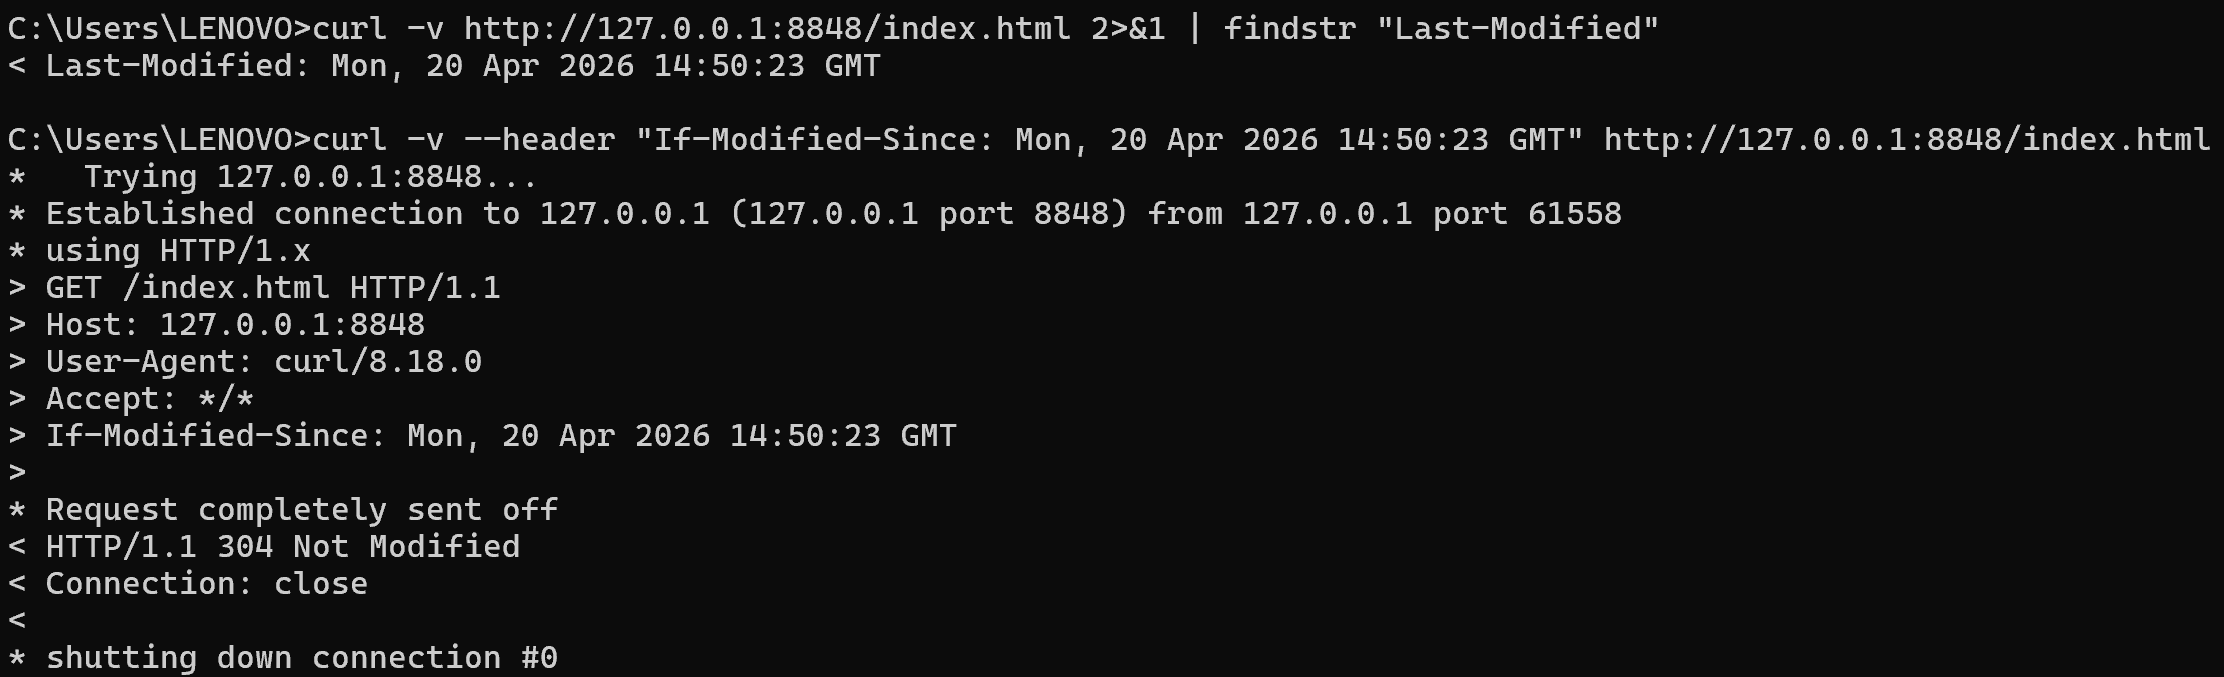
\includegraphics[width=0.8\textwidth]{09_10_lastmod_304.png}
    \caption{Last-Modified header and 304 Not Modified response}
    \label{fig:lastmod_304}
\end{figure}

\subsection{Test 11-12: Connection Keep-Alive and Close}
\textbf{Source:} Jupyter Notebook Cell 9

\textbf{Test A: Keep-Alive} - Connection header handling

\begin{verbatim}
Sent header: {'Connection': 'keep-alive'}
Returned Connection header: keep-alive
\end{verbatim}

\textbf{Test B: Connection Close}

\begin{verbatim}
Sent header: {'Connection': 'close'}
Returned Connection header: close
\end{verbatim}

\begin{figure}[H]
    \centering
    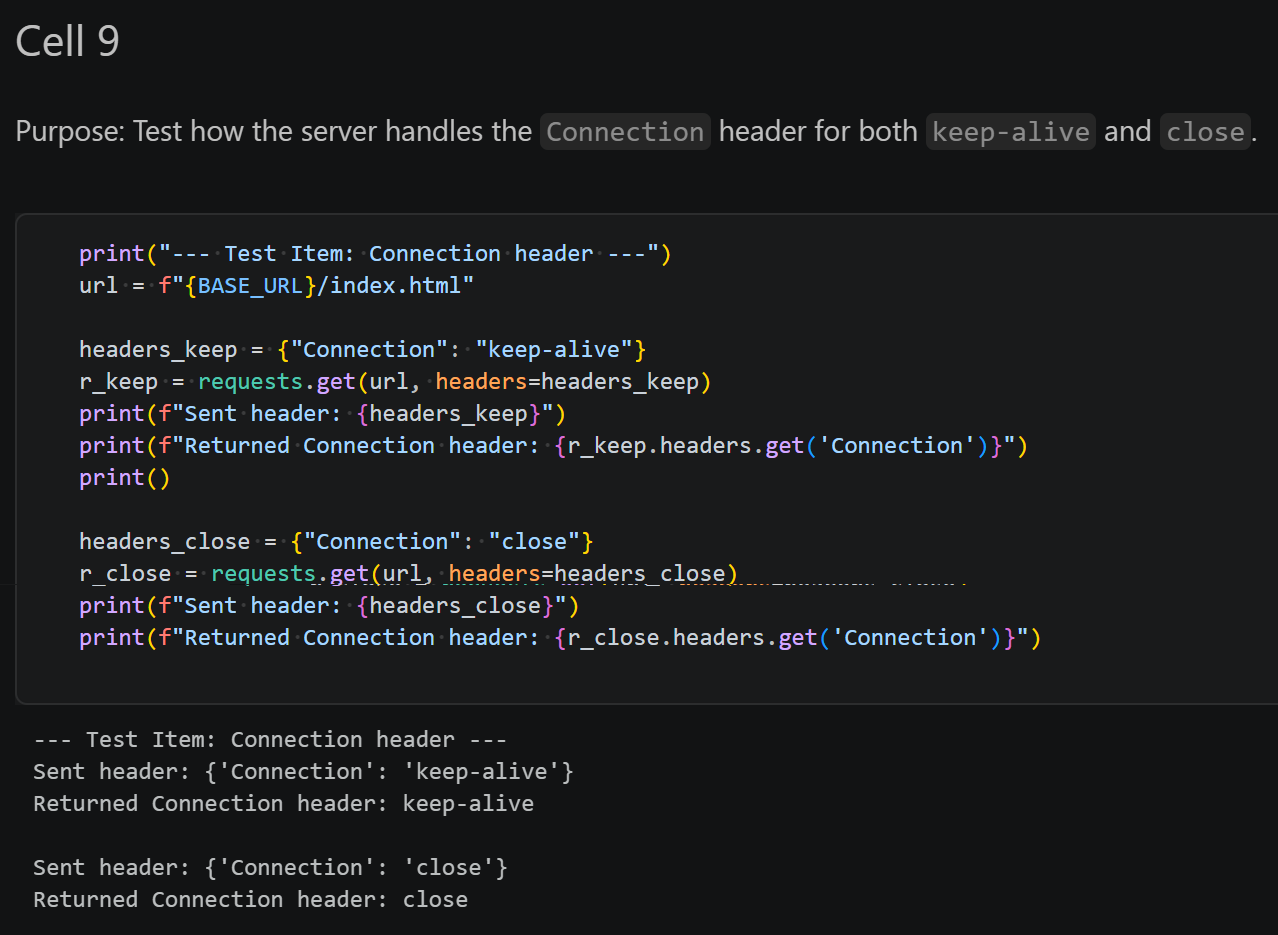
\includegraphics[width=0.8\textwidth]{11_12_keepalive_close.png}
    \caption{Connection header handling - keep-alive and close (Cell 9)}
    \label{fig:keepalive_close}
\end{figure}

\subsection{Test 13: Multi-threading Concurrent Load}
\textbf{Command:} 10 simultaneous GET requests via Python threading.

\textbf{Expected:} All 10 requests return 200 OK.

\begin{figure}[H]
    \centering
    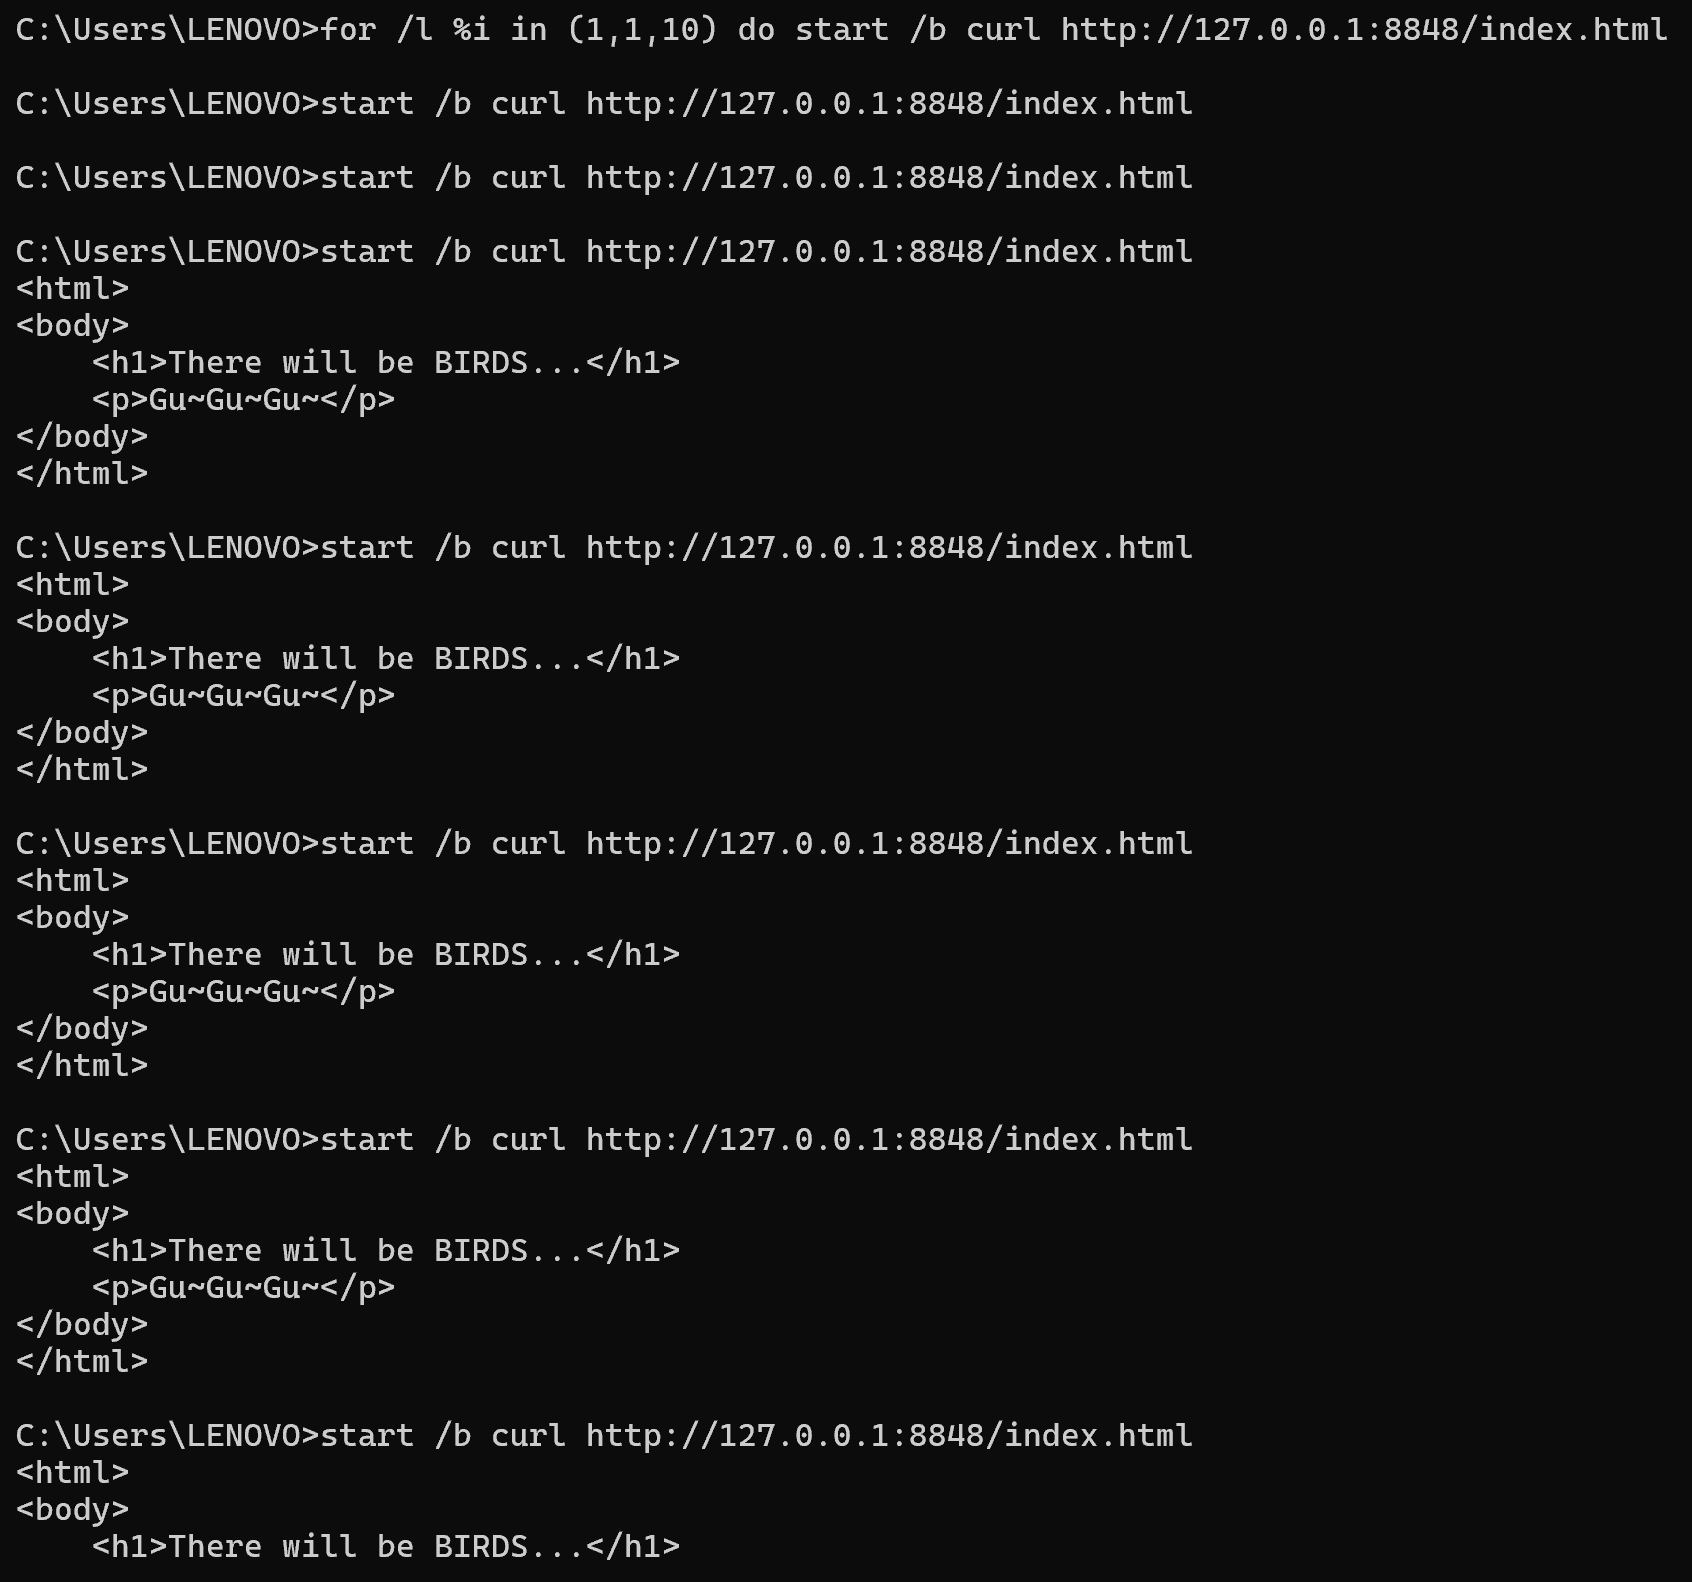
\includegraphics[width=0.8\textwidth]{13_concurrent_load.png}
    \caption{10 concurrent requests - all successful}
    \label{fig:concurrent}
\end{figure}

\subsection{Test 14: Access Log}
\textbf{Command:} \texttt{type logs\textbackslash server.log} (Windows) or \texttt{cat logs/server.log}

\textbf{Expected:} Each request recorded with IP, timestamp, request, status code.

\begin{figure}[H]
    \centering
    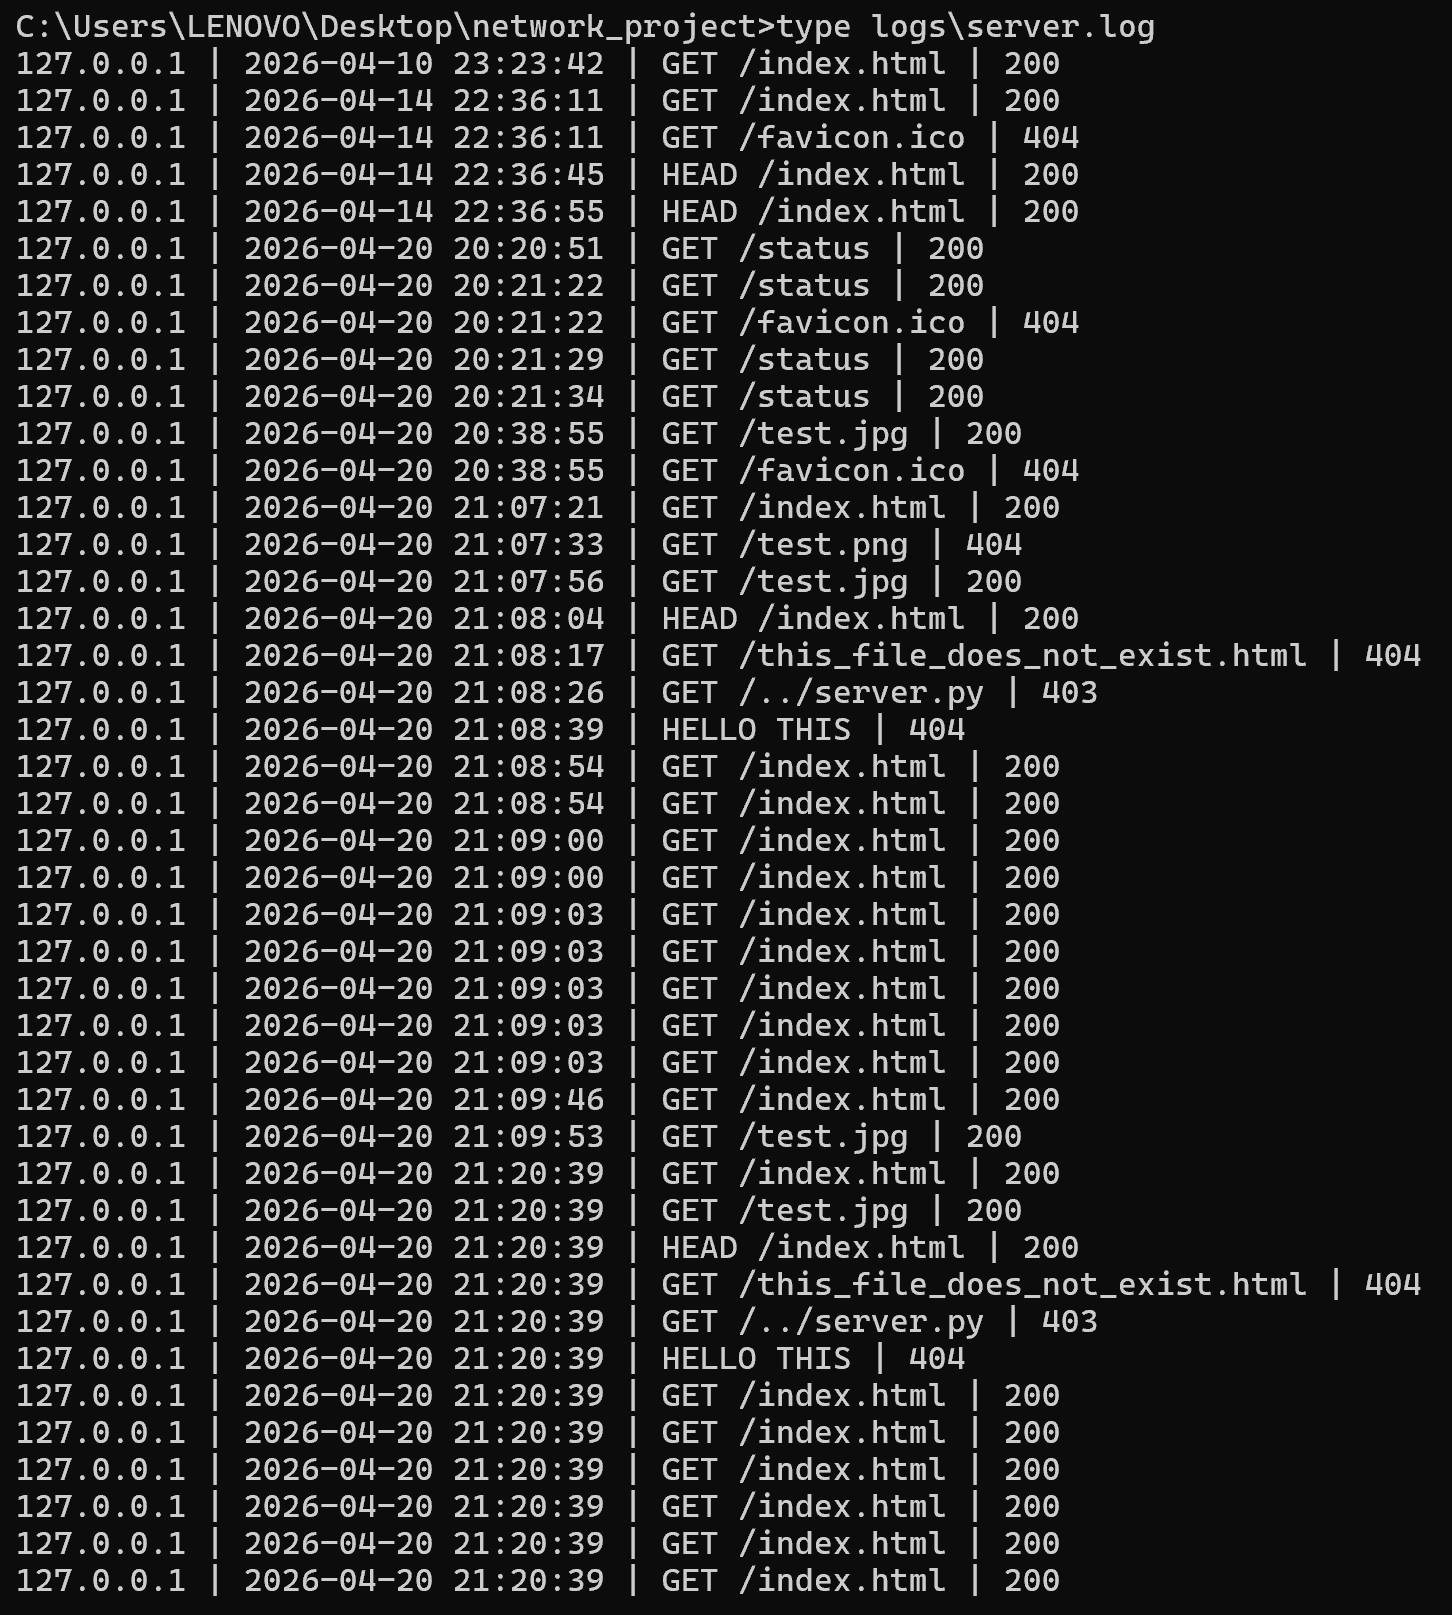
\includegraphics[width=0.8\textwidth]{14_access_log.png}
    \caption{Access log file contents}
    \label{fig:log}
\end{figure}

\subsection{Test 15: Status Dashboard}
\textbf{Method:} Visit  
\texttt{http://127.0.0.1:8848/status}
in Browser

\textbf{Expected:} HTML dashboard showing uptime, active threads, request count, recent logs.

\begin{figure}[H]
    \centering
    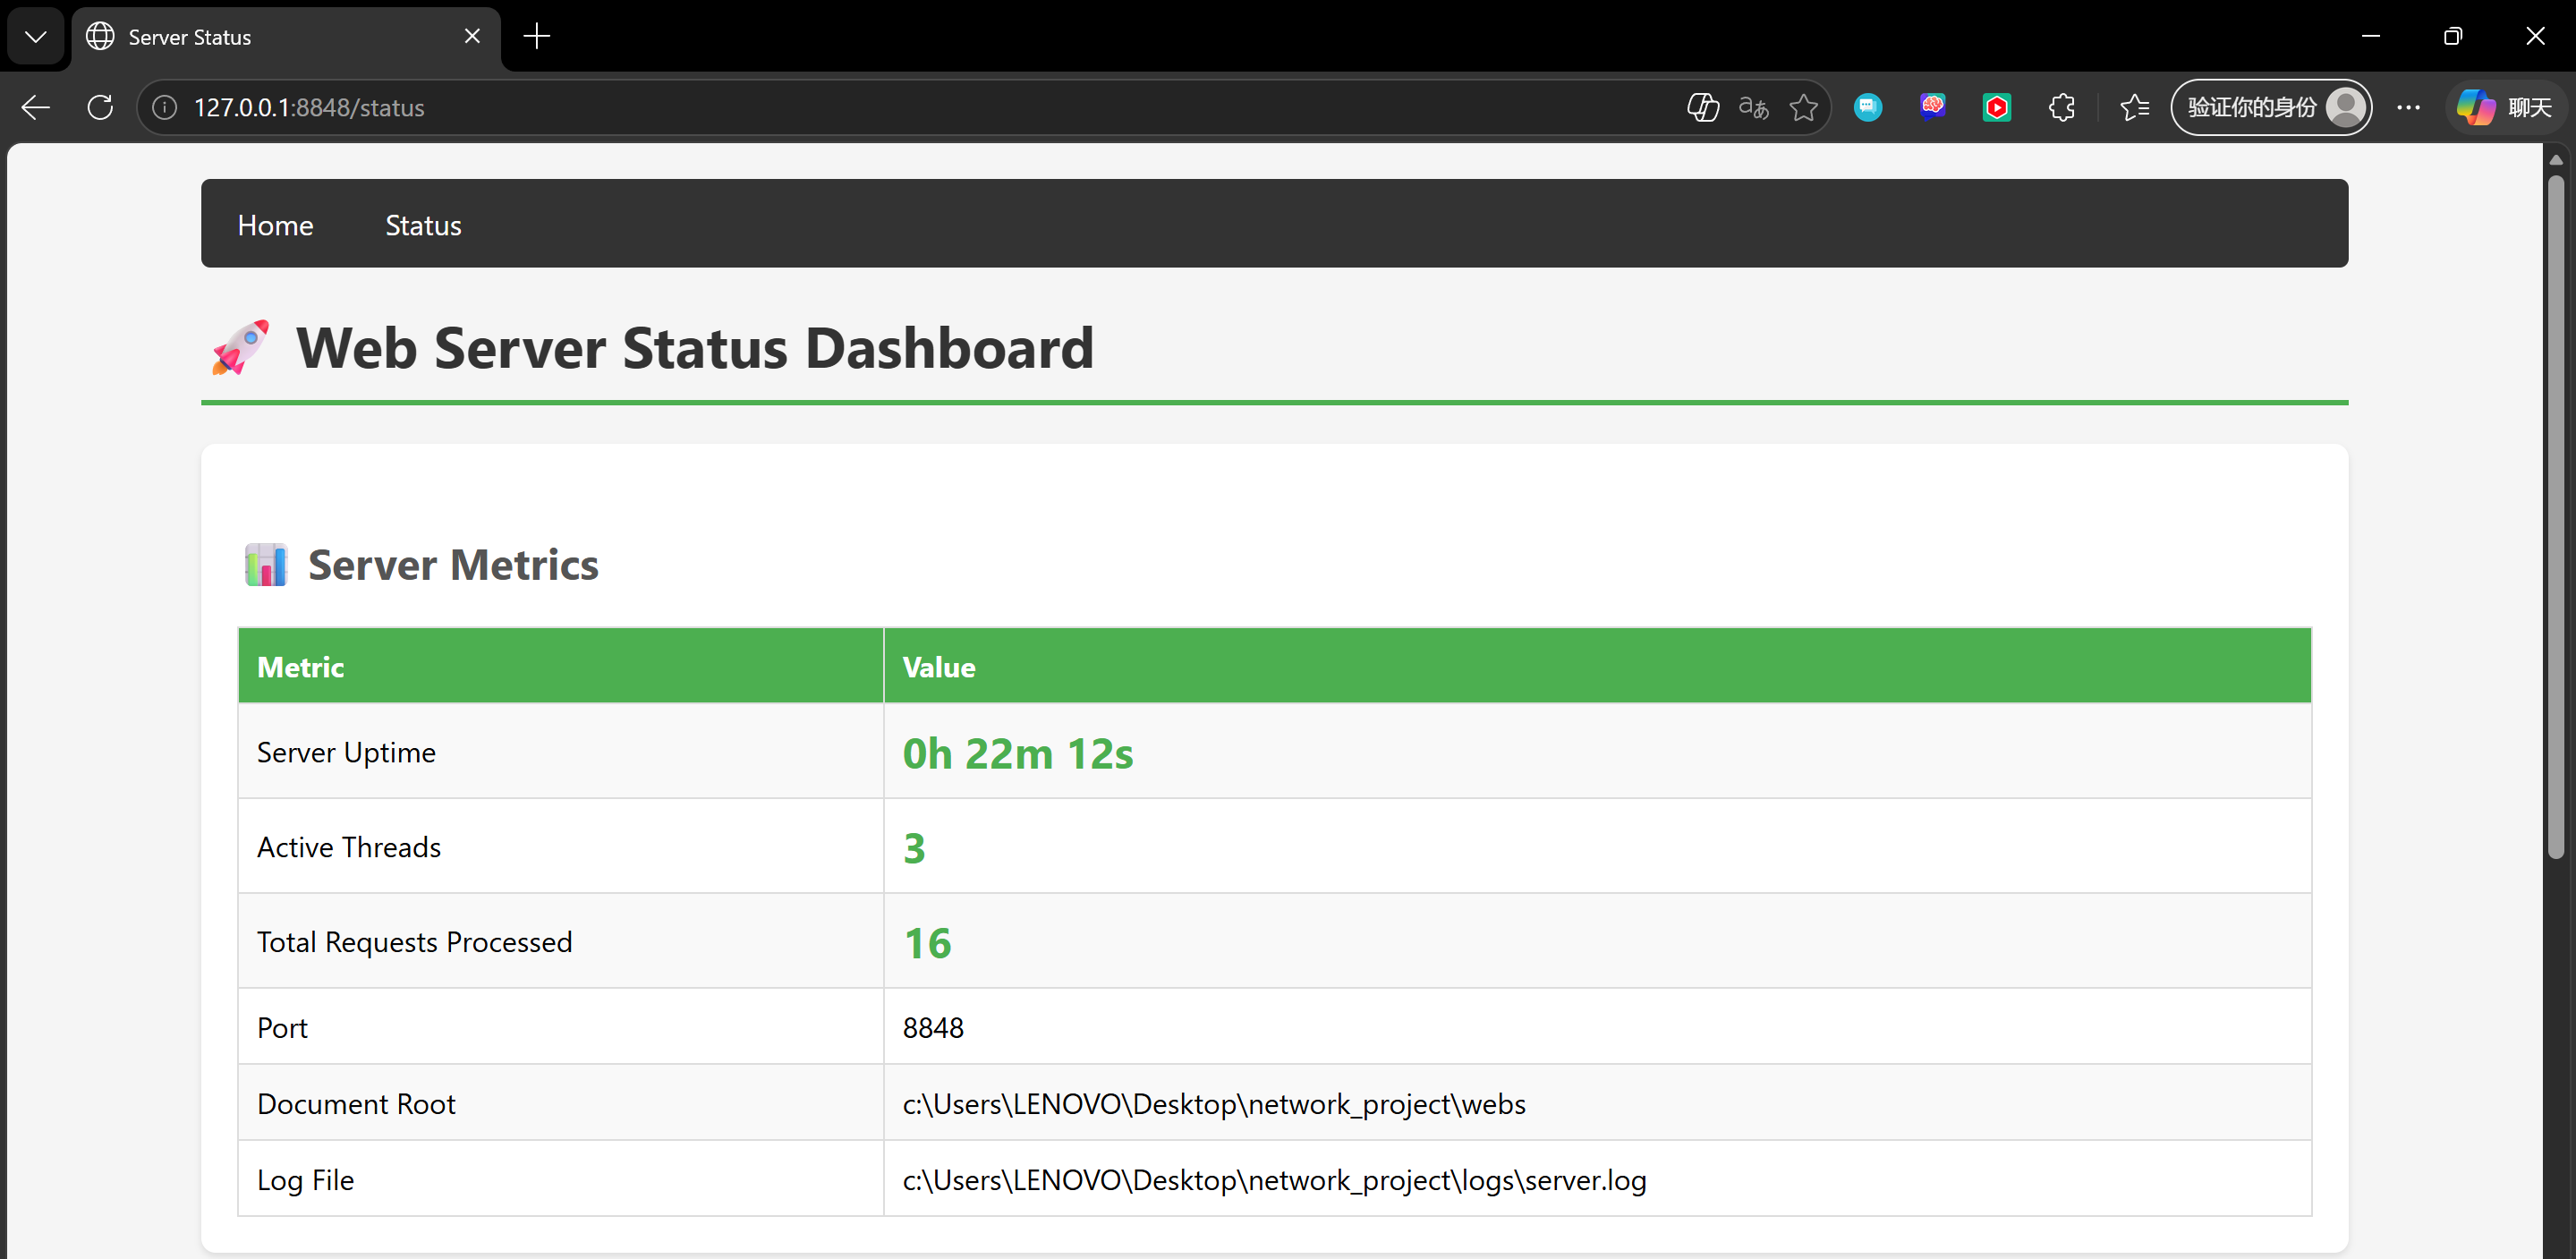
\includegraphics[width=0.8\textwidth]{15_status_dashboard.png}
    \caption{Status dashboard (browser view)}
    \label{fig:dashboard}
\end{figure}

\section{Conclusion}
Successfully implemented a fully functional multi-threaded web server supporting HTTP/1.1 features including persistent connections, cache validation, and concurrent request handling.

\appendix

\end{document}
